\documentclass{beamer}
\usepackage[utf8]{inputenc}

\usetheme{Madrid}
\usecolortheme{default}
\usepackage{amsmath,amssymb,amsfonts,amsthm}
\usepackage{txfonts}
\usepackage{tkz-euclide}
\usepackage{listings}
\usepackage{adjustbox}
\usepackage{array}
\usepackage{tabularx}
\usepackage{gvv}
\usepackage{lmodern}
\usepackage{circuitikz}
\usepackage{tikz}
\usepackage{graphicx}
\usepackage{gensymb} % For using \degree symbol
\usepackage{enumitem}

\setbeamertemplate{page number in head/foot}[totalframenumber]

% Title Information
\title{4.2.6}
\date{October 4, 2025}
\author{ADHARVAN KSHATHRIYA BOMMAGANI - EE25BTECH11003}

\begin{document}

% Title Slide
\frame{\titlepage}

% Question Slide
\begin{frame}{Question}
Find the direction and normal vectors of each of the following lines.
\begin{enumerate}[label=\textbf{4.2.\arabic*}]
    \setcounter{enumi}{5}
    \item $3x+2 = 0$
\end{enumerate}
\end{frame}

% Step 1: Normal Vector
\begin{frame}{Theoretical Solution}
The equation of a line in a 2D plane can be written in the form $\vec{n}^T \vec{x} = c$, where $\vec{n}$ is the normal vector and $\vec{x} = \myvec{ x \\ y }$.



We can rewrite the given equation $3x+2=0$ to explicitly include the $y$ term:
\begin{align*}
3x + 0y = -2
\end{align*}

This can be expressed in vector form as:
\begin{align*}
\myvec{ 3 \\ 0 }^T \myvec{ x \\ y } = -2
\end{align*}

By comparing this to the general form, we can identify the \textbf{normal vector} as:
\begin{align*}
\vec{n} = \myvec{ 3 \\ 0 }
\end{align*}
\end{frame}

% Step 2: Direction Vector
\begin{frame}{Theoretical Solution}
The direction vector $\vec{m}$ is orthogonal (perpendicular) to the normal vector $\vec{n}$. This means their dot product is zero:
\begin{align*}
\vec{m}^T \vec{n} = 0
\end{align*}

Let the direction vector be $\vec{m} = \myvec{ m_1 \\ m_2 }$. We can set up the equation:
\begin{align*}
\myvec{ m_1 & m_2 } \myvec{ 3 \\ 0 } &= 0 \\
(m_1)(3) + (m_2)(0) &= 0 \\
3m_1 &= 0 \quad \implies \quad m_1 = 0
\end{align*}

Since $m_1 = 0$, the direction vector is of the form $\myvec{ 0 \\ m_2 }$. The vector must be non-zero, so we can choose any non-zero value for $m_2$. The simplest choice is $m_2 = 1$.
\end{frame}

% Step 3: Final Answer
\begin{frame}{Theoretical Solution}
For the line $3x+2=0$:
\bigskip
\begin{itemize}
    \item \textbf{Normal Vector:} $\vec{n} = \myvec{ 3 \\ 0 }$
    \bigskip
    \item \textbf{Direction Vector:} $\vec{m} = \myvec{ 0 \\ 1 }$
\end{itemize}
\end{frame}

% Step 4: Figure
\begin{frame}{Plot}
\centering
\textbf{Illustration of the Line and Vectors:}
\begin{figure}[h!]
    \centering
    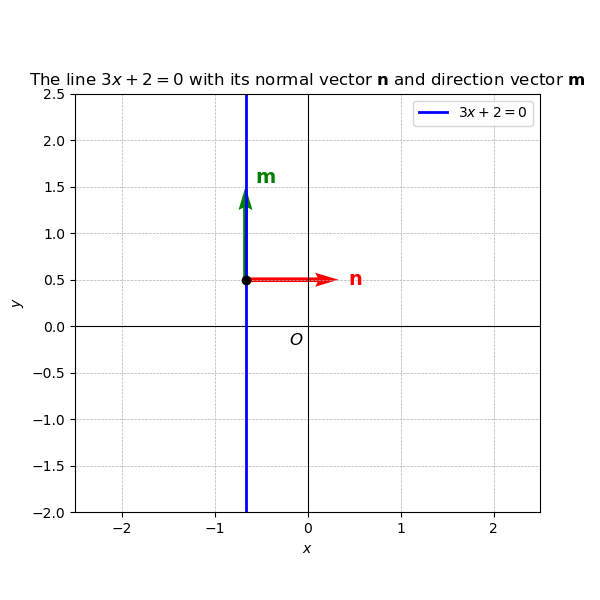
\includegraphics[width=0.7\columnwidth]{figs/fig1.png}
    \caption{The line $x = -2/3$ (blue), its normal vector $\vec{n}$ (red), and its direction vector $\vec{m}$ (green).}
\end{figure}
\end{frame}

\end{document}